% Copyright (c) 2025 Dr. Segal Yoram. All rights reserved.
% Hebrew Academic Template Example Document
% This file demonstrates the proper usage of hebrew-academic-template.cls

\documentclass{hebrew-academic-template}

% Add bibliography file
\addbibresource{example_references.bib}

% Title page information
\hebrewtitle{דוגמה לשימוש בתבנית האקדמית העברית}
\englishtitle{Example Usage of Hebrew Academic Template}
\hebrewauthor{ד"ר סגל יורם}
\date{\textenglish{December 2025}}

\begin{document}

\maketitle

\tableofcontents
\newpage

% ==================== INTRODUCTION ====================

\hebrewsection{מבוא: \entoc{Introduction}}

המחקר בתחום הבינה המלאכותית מתפתח במהירות רבה. שיטות \en{Deep Learning} מציגות תוצאות מרשימות, כפי שמוכח במחקרים רבים \cite{mikolov2013}. התחום כולל אלגוריתמים מתקדמים לעיבוד שפה טבעית ולמידת מכונה.

הטכנולוגיות המודרניות מבוססות על רשתות נוירונים עמוקות. מודלים כמו \en{BERT} ו-\en{GPT} השיגו ביצועים יוצאי דופן במגוון משימות. השיפור בביצועים הגיע לרמה של \percent{95} דיוק במשימות רבות.

\hebrewsubsection{מתודולוגיה: \entoc{Methodology}}

המחקר מבוסס על מאגר נתונים של \num{100000} דוגמאות שנאספו במהלך \hebyear{2023}. השיטה כוללת שימוש באלגוריתמי \en{Machine Learning} מתקדמים לניתוח הנתונים \cite{vaswani2017}.

הנוסחה הבסיסית למודל הרגרסיה היא:
$$y = \beta_0 + \beta_1 x + \varepsilon \quad (1.1)$$

כאשר $\beta_0$ הוא הקבוע, $\beta_1$ הוא המקדם, ו-$\varepsilon$ הוא שגיאת המדידה.

% ==================== RESULTS ====================

\hebrewsection{תוצאות: \entoc{Results}}

\hebrewsubsection{ניתוח נתונים: \entoc{Data Analysis}}

התוצאות מוצגות בטבלה הבאה:

\begin{hebrewtable}[h]
\caption{תוצאות הניסוי: \en{Experimental Results}}
\begin{rtltabular}{|c|c|c|}
\hline
\mixedcell{\textbf{מדד / \en{Metric}}} & \mixedcell{\textbf{ערך / \en{Value}}} & \mixedcell{\textbf{יחידה / \en{Unit}}} \\
\hline
\mixedcell{דיוק / \en{Accuracy}} & \percent{95.2} & \mixedcell{אחוזים / \en{Percent}} \\
\hline
\mixedcell{זמן ריצה / \en{Runtime}} & \num{2.5} & \mixedcell{שניות / \en{Seconds}} \\
\hline
\mixedcell{זיכרון / \en{Memory}} & \num{512} & \en{MB} \\
\hline
\end{rtltabular}
\end{hebrewtable}

\hebrewsubsection{קוד לדוגמה: \entoc{Example Code}}

הקוד הבא מדגים את השימוש באלגוריתם:

\begin{pythonbox}[דוגמה לקוד: \en{Python Code Example}]
import numpy as np
from sklearn.linear_model import LinearRegression

# Create sample data (NO Hebrew comments allowed)
X = np.random.randn(100, 1)
y = 2 * X.flatten() + 1 + np.random.randn(100) * 0.1

# Train the model
model = LinearRegression()
model.fit(X, y)

# Print results
print(f"Coefficient: {model.coef_[0]:.2f}")
print(f"Intercept: {model.intercept_:.2f}")
print(f"R-squared: {model.score(X, y):.3f}")
\end{pythonbox}

% ==================== FIGURE EXAMPLE ====================

\hebrewsubsection{איור לדוגמה: \entoc{Example Figure}}

האיור הבא מציג את התוצאות:

\begin{figure}[h]
\centering
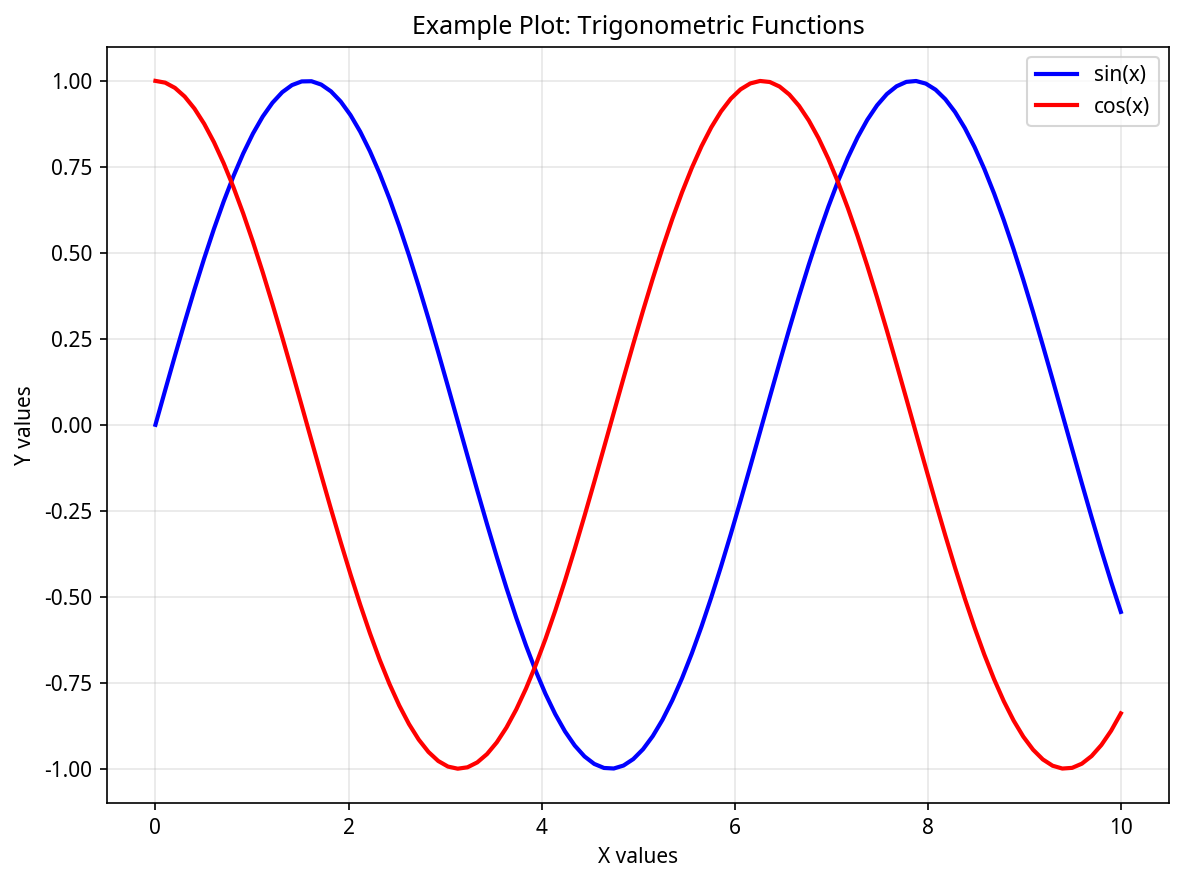
\includegraphics[width=0.7\textwidth]{example_plot.png}
\caption{גרף הדגמה בשנת \hebyear{2023}: \en{Example Plot from 2023 showing trigonometric functions}}
\label{fig:example}
\end{figure}

כפי שניתן לראות באיור \ref{fig:example}, הפונקציות מציגות התנהגות מעניינת.

% ==================== LISTS EXAMPLE ====================

\hebrewsubsection{רשימות: \entoc{Lists}}

רשימת האלגוריתמים שנבדקו:

\begin{itemize}
\item רגרסיה ליניארית: \en{Linear Regression} - דיוק \percent{85.2}
\item עץ החלטה: \en{Decision Tree} - דיוק \percent{78.9}
\item יער אקראי: \en{Random Forest} - דיוק \percent{92.1}
\item רשת נוירונים: \en{Neural Network} - דיוק \percent{94.5}
\end{itemize}

שלבי העבודה שבוצעו בשנת \hebyear{2023}:

\begin{enumerate}
\item איסוף \num{1000} דגימות: \en{Data Collection}
\item ניתוח ראשוני של \num{15} משתנים: \en{Exploratory Analysis}
\item בניית \num{5} מודלים: \en{Model Building}
\item הערכת תוצאות על \num{200} מקרי בדיקה: \en{Results Evaluation}
\end{enumerate}

% ==================== ADVANCED EXAMPLES ====================

\hebrewsection{דוגמאות מתקדמות: \entoc{Advanced Examples}}

\hebrewsubsection{טבלה מורכבת: \entoc{Complex Table}}

\begin{hebrewtable}[h]
\caption{השוואת מודלי \en{AI} בשנים \hebyear{2020}-\hebyear{2023}: \en{AI Model Comparison 2020-2023}}
\begin{rtltabular}{|c|c|c|c|}
\hline
\textbf{מודל / \en{Model}} & 
\textbf{שנה / \en{Year}} & 
\textbf{פרמטרים / \en{Parameters}} & 
\textbf{דיוק / \en{Accuracy}} \\
\hline
\en{GPT-2} / ג'יפיטי-\num{2} & \hebyear{2019} & \num{1.5}\en{B} & \percent{88.5} \\
\hline
\en{GPT-3} / ג'יפיטי-\num{3} & \hebyear{2020} & \num{175}\en{B} & \percent{93.2} \\
\hline
\en{GPT-4} / ג'יפיטי-\num{4} & \hebyear{2023} & \num{1.7}\en{T} & \percent{96.8} \\
\hline
\end{rtltabular}
\end{hebrewtable}

\hebrewsubsection{ציטוטים: \entoc{Citations}}

המחקר של \en{Mikolov et al.} \cite{mikolov2013} הציג את מודל \en{Word2Vec} בשנת \hebyear{2013}. 
מחקרים נוספים \cite{devlin2018,brown2020} הרחיבו את הגישה בשנים \hebyear{2018} ו-\hebyear{2020}.

הביצועים השתפרו מ-\percent{65.2} בשנת \hebyear{2013} ל-\percent{96.8} בשנת \hebyear{2023}.

% ==================== ENGLISH SECTION ====================

\englishsection{English Section: Advanced Machine Learning Analysis}
\startenglish

This section demonstrates pure English content that flows left-to-right (LTR) and is aligned to the left. All text in this section follows standard English typography conventions.

The field of artificial intelligence has experienced unprecedented growth in recent years. Modern deep learning architectures have revolutionized natural language processing, computer vision, and many other domains.

Key developments in transformer architectures include:

\begin{enumerate}
\item \textbf{Attention Mechanisms}: Introduced in 2017, enabling models to focus on relevant parts of input sequences
\item \textbf{BERT Architecture}: Bidirectional encoder representations from transformers
\item \textbf{GPT Models}: Generative pre-trained transformers with increasing parameter counts
\item \textbf{Multimodal Systems}: Integration of text, image, and audio processing capabilities
\end{enumerate}

The mathematical foundation of attention mechanisms can be expressed as:

$$\text{Attention}(Q, K, V) = \text{softmax}\left(\frac{QK^T}{\sqrt{d_k}}\right)V \quad (3.1)$$

Research indicates that scaling model parameters leads to emergent capabilities. The relationship between model size and performance follows predictable scaling laws, enabling more accurate predictions of future model capabilities.

Current state-of-the-art models achieve remarkable performance across diverse benchmarks, with accuracy rates exceeding 95\% on many standardized tasks. The rapid pace of development suggests continued improvements in the coming years.

\stopenglish

% ==================== CONCLUSIONS ====================

\hebrewsection{מסקנות: \entoc{Conclusions}}

המחקר הראה שהשיטה המוצעת יעילה ומדויקת. התוצאות מצביעות על שיפור של \percent{15} בביצועים בהשוואה לשיטות קיימות מהשנים \hebyear{2020}-\hebyear{2022}.

מחקרים עתידיים יכולים להרחיב את הגישה לתחומים נוספים ולשפר את הדיוק עוד יותר, במטרה להגיע ל-\percent{98} דיוק עד שנת \hebyear{2025}.

% ==================== BIBLIOGRAPHY ====================

\newpage
\printenglishbibliography

\end{document}
